\begin{figure*}[hbtp]
  \centering
  \subfigure[Our Improved Baseline approach (IBase)]{
    \label{fig:about-pruning--01}
    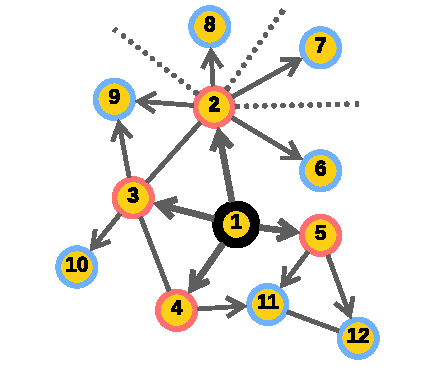
\includegraphics[width=0.31\linewidth]{out/about-pruning-01.pdf}
  }
  \subfigure[Disregard hubs with degree $> 8$ (DLH)]{
    \label{fig:about-pruning--02}
    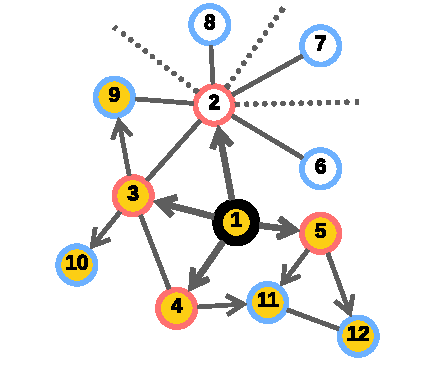
\includegraphics[width=0.31\linewidth]{out/about-pruning-02.pdf}
  }
  \subfigure[Disregard hubs with degree $> 4$ (DLH)]{
    \label{fig:about-pruning--03}
    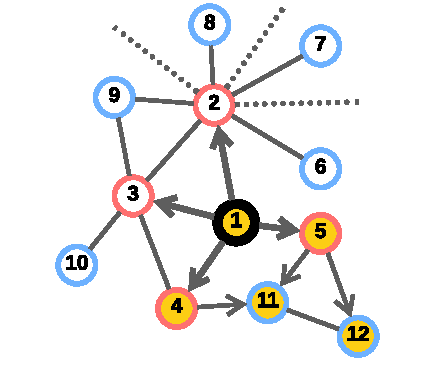
\includegraphics[width=0.31\linewidth]{out/about-pruning-03.pdf}
  } \\[-2ex]
  \caption{Illustration of our\ignore{neighborhood-based} link prediction approach which \textit{Disregards Large Hubs (DLH)}, i.e., $1^{st}$ order neighbors with high degree\ignore{(DLH)}. Here we focus on the neighborhood of vertex $1$\ignore{in the graph}, but the approach applies to each vertex in the graph. In the figure,\ignore{the current vertex} $1$ is outlined in black, its $1^{st}$ order neighbors in red, its $2^{nd}$ order neighbors in blue, and explored/traversed vertices are shown with a yellow fill. Edge directions indicate traversal, with some $2^{nd}$ order vertices omitted for simplicity (dotted edges). (a) Depicts the our \textit{Improved Baseline (IBase)} approach, which considers all $2^{nd}$ order neighbors of vertex $1$. (b) Presents our DLH approach, which considers only $2^{nd}$ order neighbors linked to $1$ through a small hub (degree $\leq 8$). This pruning reduces runtime and enhances prediction quality. (c) Illustrates DLH approach, where vertices with degree $> 4$ are considered large hubs.}
  \label{fig:about-pruning}
\end{figure*}
